% replace all text with your own text.
% in this template few examples are mention
\chapter{Methodology}
\label{ch:method} % Label for method chapter

\section{Dataset Overview and Data Exploration}

The MNIST dataset serves as a fundamental benchmark in the field of machine learning research, particularly in tasks related to image classification and recognition. This dataset consists of a collection of grayscale images of handwritten digits (0-9), each accompanied by its corresponding label indicating the digit it represents. Researchers widely utilize the MNIST dataset to evaluate the efficacy of various algorithms and techniques for digit recognition tasks.

The MNIST dataset comprises 70,000 grayscale images, divided into a training set of 60,000 images and a test set of 10,000 images. Each image is a 28x28 pixel square, resulting in a total of 784 pixels per image. These pixels represent the grayscale intensity, ranging from 0 (black) to 255 (white). Additionally, each image is associated with a label, providing ground truth information about the digit depicted in the image.

\begin{table}[htbp]
\centering
\caption{Dataset Attributes and Data Types for MNIST Dataset}
\label{tab:mnist_attributes}
\begin{tabular}{@{}lll@{}}
\toprule
\textbf{Attribute} & \textbf{Description}            & \textbf{Data Type} \\ \midrule
Image              & Handwritten digit image        & Image (28x28 pixels, grayscale) \\
Label              & Digit label                    & Integer (0 to 9) \\ 
\bottomrule
\end{tabular}
\end{table}

\subsection{Loading the Dataset} 

The MNIST dataset will be retrieved from reputable sources, such as TensorFlow or PyTorch libraries, ensuring data integrity and consistency. Both the training and testing datasets will be loaded into the research environment for further exploration.

\subsection{Visualizing Sample Images}

A random selection of sample images from the dataset will be visualized to gain insights into the characteristics of handwritten digits. These images will be displayed alongside their corresponding labels, facilitating an understanding of the dataset's content.

\begin{figure}[htbp]
  \centering
  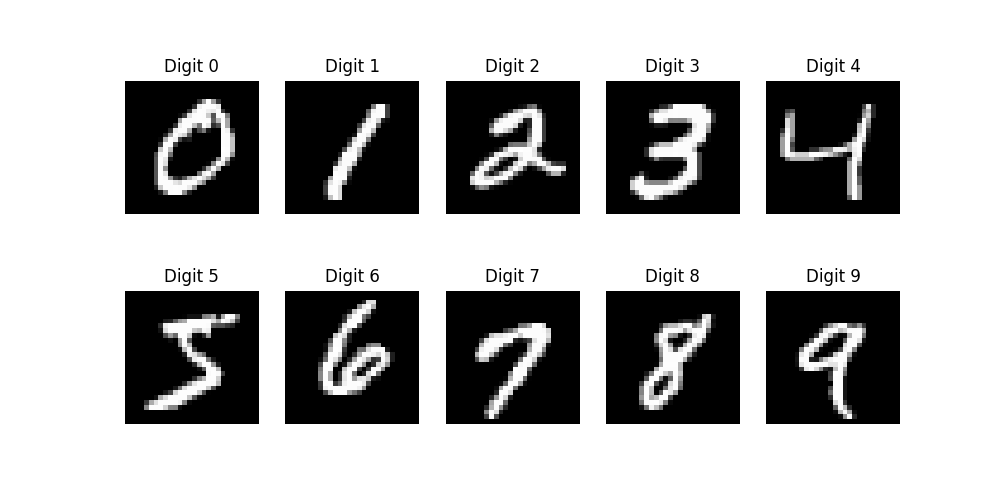
\includegraphics[width=1.0\textwidth]{figures/mnist_images.png}
  \caption{MNIST Example Images}
  \label{fig:mnist_image}
\end{figure}

\subsection{Exploring Label Distribution}

\begin{figure}[htbp]
  \centering
  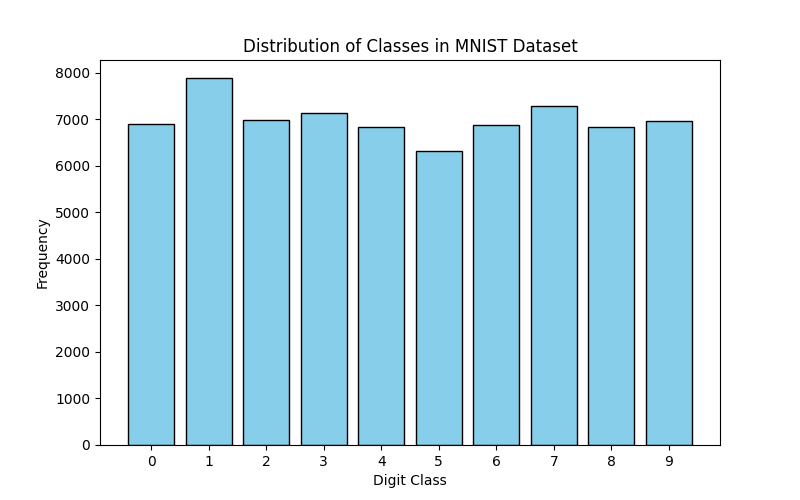
\includegraphics[width=0.7\textwidth]{figures/data_distribution.png}
  \caption{Distribution of Classes in MNIST Dataset}
  \label{fig:data_distribution}
\end{figure}

A histogram is plotted to visualize the distribution of digit labels within the training set. It is imperative to ensure that the dataset exhibits balanced label distributions, with a similar number of samples for each digit class.

\section{Data Preprocessing}

\subsection{Flatten the image data}

In the MNIST dataset, each image represents a handwritten digit and is initially structured as a 2-dimensional array (28x28 pixels). However, most machine learning algorithms, including neural networks, require input data to be in a flat, one-dimensional format. Flattening the image data involves reshaping each image into a single vector by stacking the rows of pixels one after another. This transformation simplifies the representation of the image data and allows us to treat each pixel as a separate feature. Flattening the data ensures compatibility with various machine learning models and facilitates efficient computation during training and prediction processes.

\subsection{Normalize the pixel values:}

The pixel values in the MNIST dataset represent the intensity of grayscale pixels ranging from 0 to 255. Normalizing the pixel values involves scaling them to a standard range, typically between 0 and 1 or -1 and 1. Normalization helps in stabilizing and speeding up the training process of machine learning models. It prevents certain features from dominating others due to differences in scale, thereby improving the convergence of optimization algorithms. Moreover, normalization ensures that the model's performance is not sensitive to the absolute values of the input features, making it more robust and generalizable across different datasets.

\subsection{Split the dataset into training and testing sets:}

Splitting the dataset into training and testing sets is crucial for evaluating the performance of machine learning models. The training set is used to train the model, while the testing set is used to evaluate its performance on unseen data. Additionally, it is common practice to further split the training set into a training subset and a validation set. The training subset is used for actual model training, while the validation set is used to tune hyperparameters and monitor the model's performance during training. This split helps prevent overfitting by providing an independent dataset for model evaluation and parameter tuning. Overall, splitting the dataset ensures that the model's performance estimates are reliable and generalizable to unseen data.


\subsection{Adding Noise to MNIST Images}

The add noise function provides a convenient way to induce varied levels of Gaussian noise into the MNIST dataset. This function takes two parameters: images, which represents the array of MNIST images, and noise level, which specifies the variance of the Gaussian noise to be added. The higher the noise level, the more intense the noise added to the images.

Internally, the function generates Gaussian noise with the specified variance and adds it to the input images. It ensures that the pixel values remain within the valid range of [0, 255] by clipping the values after adding noise.
By incorporating this function into the preprocessing pipeline, we can create augmented versions of the MNIST dataset with different levels of noise. These augmented datasets can help improve the model's performance, especially in scenarios where the input data may exhibit variability or uncertainty.

\section{Model Implementation}
This is the critical step where we build the model to predict handwritten digits.

\subsection{Convolutional Neural Network}

It is used for accurately classifying handwritten digits in the MNIST dataset due to their ability to effectively capture spatial patterns within images.

\begin{algorithm}
    \caption{Handwritten Digit Classification using Convolutional Neural Networks}
    \begin{algorithmic}[1]
        \Require Images $X$ and corresponding labels $y$ for training data
        \Ensure Performance metrics including accuracy, confusion matrix, precision, recall, and F1-score
        \State Create a convolutional neural network model with default architecture
        \State Train the model using the training data (images $X$ and labels $y$)
        \State Evaluate the model's performance metrics such as accuracy, confusion matrix, precision, recall, and F1-score
        \State Predict the labels for the testing data using the trained model
        \State Assess the model's performance on the testing data
        \State Calculate the performance metrics including accuracy, confusion matrix, precision, recall, and F1-score.
    \end{algorithmic}
\end{algorithm}

\subsection{Noise Function}

\begin{algorithm}
    \caption{Add Gaussian Noise to MNIST Images}
        \begin{algorithmic}[1]
            \State \textbf{Input:} MNIST images array $X_{\text{clean}}$, noise level $\sigma^2$
            \State \textbf{Output:} Noisy MNIST images array $X_{\text{noisy}}$
            \State Initialize the noise array $N \sim \mathcal{N}(0, \sigma^2)$ with the same shape as $X_{\text{clean}}$
            \State $X_{\text{noisy}} \gets X_{\text{clean}} + N$ \Comment{Add Gaussian noise to the clean images}
            \State $X_{\text{noisy}} \gets \text{clip}(X_{\text{noisy}}, 0, 1)$ \Comment{Clip values to ensure they remain between 0 and 1}
            \State \Return $X_{\text{noisy}}$
        \end{algorithmic}
\end{algorithm}

\subsection{Handwritten Digit Classification using Denoising Auto-encoder}

It is employed for enhancing the robustness of feature extraction in MNIST dataset classification tasks by reconstructing clean images from noisy inputs.


\begin{algorithm}
    \caption{Denoising Autoencoder}
        \begin{algorithmic}[1]
            \Require Noisy images $X_{\text{noisy}}$ and clean images $X_{\text{clean}}$ for training data
            \Ensure Reconstructed clean images from noisy inputs
            \State Create a denoising autoencoder model with encoder and decoder architecture
            \State Train the denoising autoencoder using the noisy images $X_{\text{noisy}}$ and their corresponding clean images $X_{\text{clean}}$
            \State Evaluate the performance of the denoising autoencoder by measuring reconstruction error
            \State Use the trained denoising autoencoder to reconstruct clean images from noisy inputs
        \end{algorithmic}
\end{algorithm}


\section{Evaluation Metrics}
In Deep learning, evaluation metrics are used to measure the performance of models, particularly in tasks like classification and regression. These metrics help in understanding how well a model is performing and are crucial for comparing different models or tuning the same model with different hyperparameters. Below is a brief description of some common evaluation metrics used in classification tasks.

\subsection{Accuracy}
Accuracy measures the fraction of predictions our model got right. It is the simplest metric for evaluation but can be misleading if the classes are imbalanced.

\[
\text{Accuracy} = \frac{\text{Number of correct predictions}}{\text{Total number of predictions}}
\]

\subsection{Confusion Matrix}
A confusion matrix is a table used to describe the performance of a classification model. It provides insights not only into the errors being made but also the types of errors that are occurring.

\[
\begin{array}{c|c|c}
 & \textbf{Predicted Positive} & \textbf{Predicted Negative} \\ \hline
\textbf{Actual Positive} & \text{True Positive (TP)} & \text{False Negative (FN)} \\ \hline
\textbf{Actual Negative} & \text{False Positive (FP)} & \text{True Negative (TN)} \\
\end{array}
\]

\subsection{Reconstruction Mean Squared Error}
Reconstruction MSE is a common metric used to evaluate the performance of image reconstruction models, particularly in contexts such as denoising or super-resolution. It measures the average squared difference between the original clean images and their reconstructed counterparts.

\[
\text{MSE} = \frac{1}{n} \sum_{i=1}^{n} (X_{\text{original}, i} - X_{\text{reconstructed}, i})^2
\]


\section{Summary}
The methodology section outlines the research approach, beginning with an overview of the MNIST dataset and exploratory data analysis. It covers data preprocessing steps like flattening and normalizing image data, along with splitting the dataset. Model implementation details for Convolutional Neural Networks (CNNs) and Denoising Autoencoders (DAEs) are provided, emphasizing their roles in digit classification and image denoising, respectively. Overall, it serves as a roadmap for conducting the research, detailing the steps involved in data preparation, model implementation, and hyperparameter optimization for accurate classification and denoising of MNIST handwritten digits.